\hypertarget{digital-signatures}{%
\section{Digital Signatures}\label{digital-signatures}}

\begin{itemize}
\tightlist
\item
  Digital Signature\\
  The result of a cryptographic transformation of data that, when
  properly implemented, provides a mechanism for verifying
  \textbf{origin authentication, data integrity and signatory
  non-repudiation.}
\item
  Non-repudiation (Nicht-leugbarkeit)\\
  A service that is used to provide assurance of the integrity and
  origin of data in such a way that the integrity and origin can be
  verified and validated by a third party as having originated from a
  specific entity in possession of the private key (i.e., the
  signatory).
\item
  Signature generation\\
  The process of using a digital signature algorithm and a
  \textbf{private key} to generate a digital signature on data.
\item
  Signature verification\\
  The process of using a digital signature algorithm and a public key to
  verify a digital signature on data.
\end{itemize}

\emph{Wir können genau dann asymmetrische Verschlüsselungsverfahren für
digitale Unterschriften verwenden, wenn die Ver- und
Entschlüsselungsverfahren des Algorithmus vertauscht werden können.}

\hypertarget{basic-idea}{%
\subsection{Basic Idea}\label{basic-idea}}

\begin{itemize}
\tightlist
\item
  Die digitale Unterschrift ist abhängig von der Nachricht und von einem
  geheimen Schlüssel
\item
  Die Signatur kann von jedem durch den öffentlichen Schlüssel überprüft
  werden
\item
  Ziel ist

  \begin{itemize}
  \tightlist
  \item
    die Authentizität des Senders sicherzustellen
  \item
    die Integrität der Nachricht (jedes Bit!) sicherzustellen
  \item
    dass der Sender die Nachricht nicht abstreiten kann (durch eine
    neutrale Stelle ist nachzuweisen, dass das Dokument vom Sender
    kommt)
  \end{itemize}
\end{itemize}

\clearpage
\hypertarget{rsa-signature}{%
\subsection{RSA-Signature}\label{rsa-signature}}

\begin{itemize}
\tightlist
\item
  Key Generation

  \begin{itemize}
  \tightlist
  \item
    Each entity creates an RSA public key and a corresponding private
    key
  \item
    The key pair used for creating digital signatures should be
    different from the key pair used for enciphering
  \end{itemize}
\item
  RSA signature generation

  \begin{itemize}
  \tightlist
  \item
    Compute $s = m^d \mod n$ (d: secret key of entity A)
  \item
    A`s signature for the message m is s.
  \end{itemize}
\item
  Verification

  \begin{itemize}
  \tightlist
  \item
    Obtain A`s authentic public key $(n, e)$
  \item
    Compute $m' = s^e \mod n$
  \item
    $m'$ must be equal to $m$
  \end{itemize}
\end{itemize}

\emph{Das Problem bei diesem Vorgehen ist die Anfrage für den
öffentlichen Schlüssel beim Sender. Was ist, wenn ein Angreiffer seinen
öffentlichen Schlüssel mit einer Man-in-the-middle-Attache unterjubelt?}

\hypertarget{attacken}{%
\subsection{Attacken}\label{attacken}}

\begin{itemize}
\tightlist
\item
  Authenticity of the public key must be secured
  (\textbf{Man-in-the-middle})

  \begin{itemize}
  \tightlist
  \item
    Cf. Certificates
  \end{itemize}
\item
  No-Message-Attacke\\
  \emph{Mit einer zufällig gewürfelter Signatur zuerst den öffentlichen
  Schlüssel anwenden und schauen, welche Nachricht dazu passt. Geht für
  kurze, nicht redundante Nachrichten wie z.B. Seriennummern.}

  \begin{itemize}
  \tightlist
  \item
    Attacker chooses an arbitrary number s and claims it to be the
    RSA-Signature of Alice
  \item
    Verification produces the message $m = s^e \mod n$
  \item
    The message m will be accepted as a signed by Alice
  \item
    Attack does not work, if the message m contains redundancy

    \begin{itemize}
    \tightlist
    \item
      e.g.~natural language
    \item
      A randomly chosen s will produce a message m that does not make
      sense
    \item
      If there is no redundancy (e.g.~m can be an arbitrary number),
      redundancy must be enforced by a redundancy function R(m), e. g. m
      = 123, R(m) = 123123
    \end{itemize}
  \end{itemize}
\item
  Multiplicative property of RSA\\
  \emph{Die verschlüsselten Nachrichten lassen sich miteinander
  multiplizieren. Das heisst, wenn man die Signatur von $m_1$ und $m_2$ kennt,
  kennt man auch die Signatur von $m = m_1 * m_2$.}

  \begin{itemize}
  \tightlist
  \item
    $s_1 = m_1^d \mod n, s_2 = m_2d \mod n \Rightarrow s = (m1 * m2 )^d \mod n$
  \item
    $s$ is the signature corresponding to the message $m1 * m2$
  \item
    Given two valid signatures, we can easily produce a third valid
    signature
  \item
    Chosen-Message-Attack

    \begin{itemize}
    \tightlist
    \item
      Attacker would like Alice to sign message $m$
    \item
      He chooses any $m_1$ with $ggT(m_1 ,n) = 1$
    \item
      He computes $m_2 = m * m_1-1 \mod n$
    \item
      He asks Alice to sign $m_1$ und $m_2 \Rightarrow s_1$ , $s_2$
    \item
      He computes $s$ = $s_1 * s_2$
    \end{itemize}
  \item
    Attack does not work if $m$ contains redundancy

    \begin{itemize}
    \tightlist
    \item
      e.g.~natural language
    \end{itemize}
  \end{itemize}
\end{itemize}

\hypertarget{hash-funktionen}{%
\subsection{Hash Funktionen}\label{hash-funktionen}}

Eine Hash-Funktion ist eine Funktion, die eine beliebig lange
Bit-Sequenz empfängt und einen Hash-Wert liefert, welcher immer eine
fixe Anzahl Bits hat.

\begin{tcolorbox}[colback=red!5!white,colframe=red!75!black]
    $h: \{0,1\}^x \Rightarrow \{0,1\}^n$
\end{tcolorbox}

\textbf{Hash functions can never be injective}\\
Eine Funktion ist dann injectiv, wenn ich aus dem Input eindeutig auf
das Resultat schliessen kann.

\textbf{Collision}\\
Zwei verschiedene Eingangswerte, die genau den gleichen Hash-Wert
ergeben.

\hypertarget{kryptografische-hash-funktionen}{%
\subsubsection{Kryptografische Hash
Funktionen}\label{kryptografische-hash-funktionen}}

\begin{enumerate}
\def\labelenumi{\arabic{enumi}.}
\tightlist
\item
  Preimage Resistance\\
  Das Resultat nennt man Image. Wenn die Hash-Funktion Preimage Resistant ist, ist es nicht  praktikable, aus dem Resultat ein passender Input (Preimage) zu berechnen. $\Rightarrow$ Einwegfunktion.
  \begin{itemize}
\tightlist
\item
  For a given hash value, it is difficult to find a corresponding input
  string
\item
  $h(m)$ is a one-way function
\end{itemize}

\item
  Second-Preimage Resistance\\
  Gegeben ist $m_1$. Es ist unmöglich, einen zweiten Input aus dem Hash-Wert zu finden.
  \begin{itemize}
\tightlist
\item
  Given an input $m_1$ , it is difficult to find a second input $m_2$ such
  that $h(m_1) = h(m_2)$
\item
  Also called weak collision resistance
\end{itemize}

\item
  Collision Resistance (Härteste Bedingung, weil keine Vorgaben)\\
 Es ist nichts vorgegeben. Finde zwei beliebige Nachrichten $m_1$ \& $m_2$, die denselben Hashwert haben. Wenn das nicht möglich ist, ist die Hash-Funktion Collision Resistant.

\begin{itemize}
\tightlist
\item
  It is difficult to find two different input strings $m_1$ and $m_2$ such
  that $h(m_1) = h(m_2)$
\item
  Also called strong collision resistance
\end{itemize}
 
\end{enumerate}


\hypertarget{message-authentication-codes}{%
\subsection{Message Authentication
Codes}\label{message-authentication-codes}}

Also called \textbf{«parametrized hash function»}

Zur Berechnung des Hash-Wertes braucht es zusätzlich noch einen geheimen
Parameter $k$. Wenn diese Message Authentication Code stimmt, kann ich mir
sicher sein, dass dies von jemandem berechnet wurde, der das Geheimnis
kennt.

\hypertarget{signature-with-hash-function}{%
\subsection{Signature with Hash
Function}\label{signature-with-hash-function}}

Statt die ganze Nachricht zu signieren, berechne ich den Hash-Wert der
Nachricht und signiere diesen. Dies ist viel effizienter.

\begin{figure}[H]
\centering
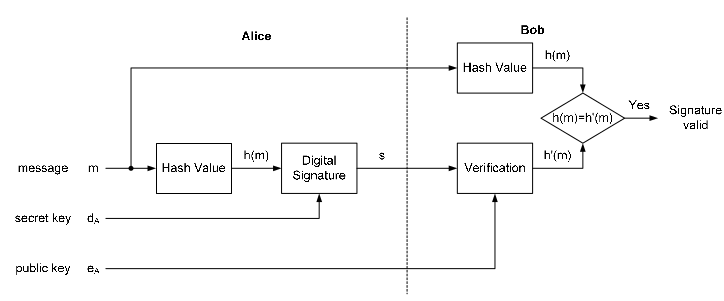
\includegraphics[width=0.8\textwidth]{figures/digitanSignatureWithHash.png}
\caption{Digital Signature with Hash Function}
\end{figure}

\hypertarget{vorteile}{%
\subsubsection{Vorteile}\label{vorteile}}

\begin{itemize}
\tightlist
\item
  Anstelle von langen Nachrichten muss ich nur kurze Hash-Werte
  unterschreiben
\item
  Die No-Message-Attacke funktioniert nicht

  \begin{itemize}
  \tightlist
  \item
    Mit der Signatur s kann der Angreiffer ein Hash-Wert generieren
  \item
    Der Angreiffer kann aber keine Nachricht generieren, die den
    erwünschten Hash ergibt $\Rightarrow$ da Einwegfunktion
  \end{itemize}
\item
  Auch die multiplikative Eigenschaft von RSA kann man nicht mehr
  ausnützen

  \begin{itemize}
  \tightlist
  \item
    Die Nachricht m ist nämlich nicht bekannt
  \end{itemize}
\item
  Die Nachricht kann nicht durch eine andere Nachricht ersetzt werden
\end{itemize}

\hypertarget{digital-signature-algorithm---dsa}{%
\subsection{Digital Signature Algorithm -
DSA}\label{digital-signature-algorithm---dsa}}

\subsubsection{Key Generation}
\begin{figure}[H]
\centering
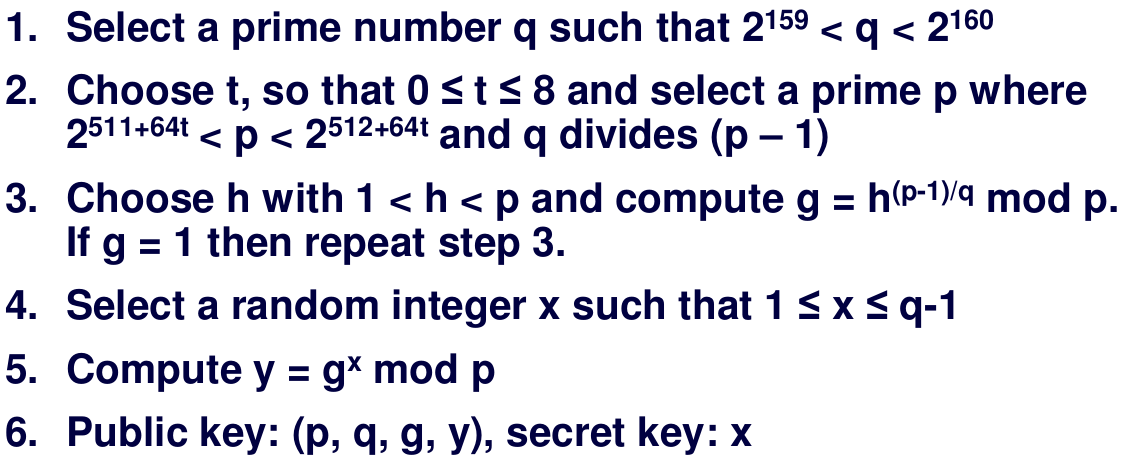
\includegraphics[width=0.6\textwidth]{figures/DSS-Keygeneration.png}
\caption{DSS Keygeneration}
\end{figure}


\subsubsection{DSA Signature Generation}:\\
\begin{figure}[H]
\centering
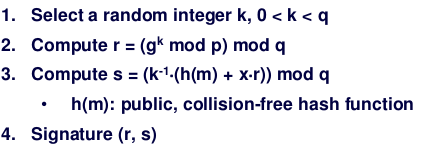
\includegraphics[width=0.6\textwidth]{figures/DSA_signature.png}
\caption{DSA Signature Generation}
\end{figure}

\subsubsection{DSA Signature Verification}:\\
\begin{figure}[H]
\centering
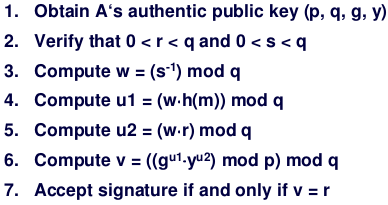
\includegraphics[width=0.6\textwidth]{figures/DSA_verification.png}
\caption{DSA Signature Verification}
\end{figure}

\hypertarget{public-key-infrastructure---pki}{%
\subsection{Public Key Infrastructure -
PKI}\label{public-key-infrastructure---pki}}

\begin{itemize}
\tightlist
\item
  Stellt folgende Eigenschaften sicher

  \begin{itemize}
  \tightlist
  \item
    Who is the owner of a public key?
  \item
    Is the public key still valid?
  \item
    What can it be used for?
  \end{itemize}
\item
  Idee: Usage of digital certificates

  \begin{itemize}
  \tightlist
  \item
    Digitally signed electronic data that can be used to verify the
    authenticity of objects
  \item
    Similiar to a passport
  \end{itemize}
\item
  But: Who should sign the certificate?

  \begin{itemize}
  \tightlist
  \item
    We need a trusted third party that issues digital certificates
  \item
    Certification-Authority (CA)
  \end{itemize}
\end{itemize}

\begin{figure}[H]
\centering
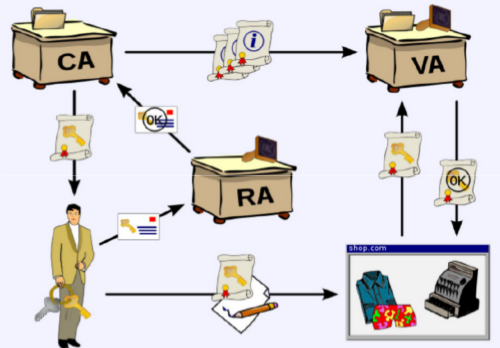
\includegraphics[width=0.4\textwidth]{figures/elementsPKI.png}
\caption{Elements of a PKI}
\end{figure}

\begin{itemize}
\tightlist
\item
  Wenn ich mich registrieren lassen möchte, muss ich mich bei einer
  Registration Authority authentifizieren und registrieren.
\item
  Von der Certification Authority bekomme ich dann ein Zertifikat, das
  ich an andere weitergeben kann, um meine Identität zu beweisen.
\item
  Andere Benutzer, die mich überprüfen möchten, können mein Zertifikat
  bei der Validation Authority überprüfen lassen.
\end{itemize}

\hypertarget{trust-models}{%
\subsection{Trust Models}\label{trust-models}}

\begin{itemize}
\tightlist
\item
  Direct Trust\\
  Ich kenne diese Person persönlich oder direkt
\item
  Hierarchical Trust\\
  Mittels PKI
\item
  Web of Trust \\
  Mein Freund ist auch dein Freund.\\
  \begin{itemize}
      \item
  Each user can sign a key. Thereby the key becomes valid.
\item
  A user should only sign a key if he is 100\% assured of its
  authenticity.
\item
  Each user \textbf{can define the level of trust} that the key`s owner
  can serve as certifier of other` keys.
  \begin{itemize}
  \tightlist
  \item
    untrusted\\
    Ich kenne denjenigen gar nicht.
  \item
    marginal\\
    Ich kenne die zwar, ich kann denen aber nicht vollumfänglich
    glauben.
  \item
    trusted\\
    Denen traue ich voll und ganz.
  \end{itemize}
  \end{itemize}

\end{itemize}


\clearpage